\chapter{Fase C: Arsitektur Data}

\section{Tujuan}
Tujuan dari fase ini adalah untuk mengembangkan Arsitektur Data Target yang memungkinkan Arsitektur Bisnis dan Visi Arsitektur dapat tercapai, sambil menangani Permintaan Pekerjaan Arsitektur dan \textit{concerns} dari para \textit{stakeholder}. Selain itu, fase ini bertujuan untuk mengidentifikasi komponen Peta Jalan Arsitektur berdasarkan kesenjangan antara Arsitektur Data Dasar dan Arsitektur Data Target.

\section{Input (1)}
Input yang digunakan dalam fase ini meliputi:
\begin{enumerate}
	\item Permintaan Pekerjaan Arsitektur
	\item Penilaian Kapabilitas
	\item Rencana Komunikasi
	\item Model Organisasi untuk Arsitektur Perusahaan
	\item Kerangka Kerja Arsitektur yang Disesuaikan
	\item Prinsip Data, jika ada
	\item Pernyataan Pekerjaan Arsitektur
	\item Draf Spesifikasi Kebutuhan Arsitektur, mencakup:
	\begin{enumerate}
		\item Hasil Analisis Kesenjangan
		\item Kebutuhan teknis relevan lainnya
	\end{enumerate}
	\item Visi Arsitektur
	\item Repositori Arsitektur
	\item Draf Dokumen Definisi Arsitektur, mencakup:
	\begin{enumerate}
		\item Arsitektur Bisnis Dasar (rinci)
		\item Arsitektur Bisnis Target (rinci)
		\item Arsitektur Data Dasar (garis besar)
		\item Arsitektur Data Target (garis besar)
		\item Arsitektur Aplikasi Dasar (garis besar)
		\item Arsitektur Aplikasi Target (garis besar)
		\item Arsitektur Teknologi Dasar (garis besar)
		\item Arsitektur Teknologi Target (garis besar)
	\end{enumerate}
	\item Komponen Arsitektur Bisnis dari Peta Jalan Arsitektur
\end{enumerate}

\section{Langkah-langkah}
Langkah-langkah yang diambil dalam fase ini meliputi:
\begin{enumerate}
	\item Memilih model referensi, sudut pandang, dan alat
	\item Mengembangkan Deskripsi Arsitektur Data Dasar
	\item Mengembangkan Deskripsi Arsitektur Data Target
	\item Melakukan Analisis Kesenjangan
	\item Menentukan komponen peta jalan kandidat
	\item Menyelesaikan dampak pada Lanskap Arsitektur
	\item Melakukan tinjauan formal dari pemangku kepentingan
	\item Menyelesaikan Arsitektur Data
	\item Membuat Dokumen Definisi Arsitektur
\end{enumerate}

\subsection*{Contoh:}
Langkah-langkah yang diambil dalam fase ini meliputi:
\begin{enumerate}
	\item Memilih model referensi, sudut pandang, dan alat
	\begin{itemize}
		\item Contoh: Memilih model referensi pedagogis seperti Community of Inquiry (CoI) untuk pembelajaran hybrid, dengan sudut pandang dari dosen dan mahasiswa, serta alat seperti Moodle atau Google Classroom untuk manajemen kursus.
	\end{itemize}
	\item Mengembangkan Deskripsi Arsitektur Data \textit{Baseline}
	\begin{itemize}
		\item Contoh: Membuat peta data yang mencakup informasi tentang interaksi mahasiswa dalam lingkungan belajar daring dan luring, seperti data kehadiran dan partisipasi dalam diskusi.
	\end{itemize}
	\item Mengembangkan Deskripsi Arsitektur Data Target
	\begin{itemize}
		\item Contoh: Merancang sistem yang mendukung analitik pembelajaran untuk mengevaluasi keterlibatan dan kemajuan mahasiswa, termasuk pengintegrasian data dari platform pembelajaran dan sistem manajemen akademik.
	\end{itemize}
	\item Melakukan Analisis Kesenjangan
	\begin{itemize}
		\item Contoh: Menganalisis kesenjangan antara praktik pengajaran saat ini dan kebutuhan untuk model pembelajaran hybrid, seperti kurangnya data tentang keterlibatan mahasiswa dalam sesi tatap muka versus daring.
	\end{itemize}
	\item Menentukan komponen peta jalan kandidat
	\begin{itemize}
		\item Contoh: Mengidentifikasi proyek-proyek pengembangan kursus hybrid, seperti pelatihan dosen dalam penggunaan teknologi pembelajaran dan pengembangan materi pembelajaran yang dapat diakses secara daring.
	\end{itemize}
	\item Menyelesaikan dampak pada Lanskap Arsitektur
	\begin{itemize}
		\item Contoh: Menganalisis dampak transisi ke pembelajaran hybrid pada infrastruktur TI universitas dan kesiapan dosen untuk mengajar dalam format ini.
	\end{itemize}
	\item Melakukan tinjauan formal dari pemangku kepentingan
	\begin{itemize}
		\item Contoh: Mengadakan forum diskusi dengan dosen, mahasiswa, dan staf administrasi untuk meninjau arsitektur pembelajaran hybrid dan mengumpulkan masukan tentang tantangan yang dihadapi.
	\end{itemize}
	\item Menyelesaikan Arsitektur Data
	\begin{itemize}
		\item Contoh: Finalisasi desain arsitektur data yang mendukung evaluasi efektivitas pembelajaran hybrid dengan memperhitungkan umpan balik dari pemangku kepentingan dan analisis data yang ada.
	\end{itemize}
	\item Membuat Dokumen Definisi Arsitektur
	\begin{itemize}
		\item Contoh: Menyusun dokumen definisi arsitektur yang merinci struktur dan proses pembelajaran hybrid, kebijakan penggunaan teknologi, dan protokol untuk mengukur hasil pembelajaran.
	\end{itemize}
\end{enumerate}


\section{Output}
Output dari fase ini mencakup:
\begin{enumerate}
	\item Pernyataan Pekerjaan Arsitektur, diperbarui sesuai kebutuhan
	\item Prinsip-prinsip data yang divalidasi, atau prinsip-prinsip data baru
	\item Draf Dokumen Definisi Arsitektur dengan konten yang diperbarui
	\item Spesifikasi Kebutuhan Arsitektur yang telah didesain, termasuk yang telah diperbarui
	\item Komponen Arsitektur Data dari Peta Jalan Arsitektur
\end{enumerate}

\subsection{Output}
Output dari fase ini mencakup:
\begin{enumerate}
	\item Pernyataan Pekerjaan Arsitektur, diperbarui sesuai kebutuhan
	\begin{itemize}
		\item Contoh: Dokumen Pernyataan Pekerjaan Arsitektur yang merinci tanggung jawab dan tugas tim dalam mengembangkan lingkungan belajar hybrid, termasuk penyesuaian terhadap kebutuhan teknologi yang muncul selama proses pengajaran.
	\end{itemize}
	\item Prinsip-prinsip data yang divalidasi, atau prinsip-prinsip data baru
	\begin{itemize}
		\item Contoh: Prinsip data yang divalidasi untuk menjaga kerahasiaan data mahasiswa dan memastikan aksesibilitas konten pembelajaran secara adil, serta penambahan prinsip baru mengenai penggunaan data analitik untuk meningkatkan pengalaman belajar mahasiswa.
	\end{itemize}
	\item Draf Dokumen Definisi Arsitektur dengan konten yang diperbarui
	\begin{itemize}
		\item Contoh: Draf Dokumen Definisi Arsitektur yang mencakup detail terbaru mengenai platform pembelajaran yang digunakan, prosedur pengajaran hybrid, dan mekanisme evaluasi yang terintegrasi antara pembelajaran daring dan luring.
	\end{itemize}
	\item Spesifikasi Kebutuhan Arsitektur yang telah didesain, termasuk yang telah diperbarui
	\begin{itemize}
		\item Contoh: Spesifikasi kebutuhan yang mencakup alat dan teknologi yang diperlukan untuk mendukung pembelajaran hybrid, seperti perangkat lunak untuk pengelolaan kursus dan sistem umpan balik mahasiswa yang efektif.
	\end{itemize}
	\item Komponen Arsitektur Data dari Peta Jalan Arsitektur
	\begin{itemize}
		\item Contoh: Komponen arsitektur data yang menggambarkan struktur sistem penyimpanan data untuk pembelajaran hybrid, termasuk database untuk menyimpan catatan kehadiran, partisipasi dalam diskusi, dan hasil evaluasi, serta integrasi data dari berbagai platform yang digunakan.
	\end{itemize}
\end{enumerate}

\section{Prinsip Data}
Beberapa prinsip data yang dipegang dalam fase ini adalah:
\begin{enumerate}
	\item \textbf{Data adalah Aset}. Data adalah aset yang memiliki nilai bagi perusahaan dan dikelola sesuai dengan itu.
	\item \textbf{Data dapat dibagikan}. Pengguna dapat mengakses data yang diperlukan untuk melaksanakan tugas mereka; oleh karena itu, data dibagikan di seluruh fungsi dan organisasi perusahaan.
	\item \textbf{Data yang dapat diakses}. Data dapat diakses oleh pengguna untuk menjalankan fungsi mereka.
	\item \textbf{Definisi Kosakata dan Data yang Dibagikan}. Data didefinisikan secara konsisten di seluruh perusahaan, dan definisi tersebut dapat dipahami serta tersedia untuk semua pengguna.
	\item \textbf{Keamanan Data}. Data dilindungi dari penggunaan dan pengungkapan yang tidak sah. Selain aspek tradisional dari klasifikasi keamanan nasional, ini termasuk tetapi tidak terbatas pada perlindungan sebelum keputusan, informasi sensitif, pemilihan sumber sensitif, dan informasi kepemilikan.
\end{enumerate}

\section{Katalog, Matriks, dan Diagram Arsitektur Data}
Dalam fase ini, berbagai katalog, matriks, dan diagram yang digunakan meliputi:
\begin{table}[ht]
	\begin{tabular}{|c|c|c|}
		\hline
		\textbf{Katalog} & \textbf{Matriks} & \textbf{Diagram} \\ \hline
		Katalog Entitas Data/Komponen & Matriks Entitas Data/Fungsi Bisnis & Diagram Data Konseptual \\
		& Matriks Aplikasi/Data & Diagram Data Logis \\
		& & Diagram Penyebaran Data \\
		& & Diagram Siklus Hidup Data \\
		& & Diagram Keamanan Data \\
		& & Diagram Migrasi Data \\ \hline
	\end{tabular}
\end{table}

\section{Komponen Dokumen Definisi Arsitektur}
\label{sec:dokumen_definisi_arsitektur_data}
Topik yang harus dibahas dalam Dokumen Definisi Arsitektur yang terkait dengan Arsitektur Data adalah sebagai berikut:
\begin{itemize}
	\item Arsitektur Data Baseline, jika memungkinkan
	\item Arsitektur Data Target, termasuk model untuk data bisnis, data logis, dan proses manajemen data, serta matriks Entitas Data/Fungsi Bisnis
	\item Pandangan Arsitektur Data yang sesuai dengan sudut pandang yang dipilih, yang mengatasi kekhawatiran pemangku kepentingan kunci
\end{itemize}

\subsection*{Contoh:}
\begin{itemize}
	\item \textbf{Arsitektur Data Baseline, jika memungkinkan} \\
	Contoh: Pada fase awal implementasi hybrid learning, universitas mengumpulkan data mengenai penggunaan platform pembelajaran daring (LMS) dan kehadiran mahasiswa dalam pertemuan tatap muka. Data baseline ini mencakup statistik tentang frekuensi akses mahasiswa ke materi pembelajaran, tingkat partisipasi dalam diskusi online, dan kehadiran dalam kelas fisik. 
	
	\item \textbf{Arsitektur Data Target, termasuk model untuk data bisnis, data logis, dan proses manajemen data, serta matriks Entitas Data/Fungsi Bisnis} \\
	Contoh: Universitas menetapkan Arsitektur Data Target yang mencakup model untuk pengelolaan data mahasiswa, dosen, dan kurikulum. Model ini memetakan hubungan antara entitas seperti mahasiswa, kursus, dan dosen. Misalnya, matriks Entitas Data/Fungsi Bisnis menunjukkan bagaimana data tentang mahasiswa (seperti nilai dan kehadiran) digunakan untuk meningkatkan pengalaman belajar dalam konteks hybrid, misalnya, melalui pengembangan materi yang sesuai untuk pembelajaran daring dan tatap muka.
	
	\item \textbf{Pandangan Arsitektur Data yang sesuai dengan sudut pandang yang dipilih, yang mengatasi kekhawatiran pemangku kepentingan kunci} \\
	Contoh: Dalam konteks hybrid learning, pandangan arsitektur data mencakup perspektif pemangku kepentingan seperti mahasiswa, dosen, dan pengelola pendidikan. Misalnya, mahasiswa mungkin mengkhawatirkan aksesibilitas materi pembelajaran secara daring, sedangkan dosen mungkin fokus pada bagaimana data kehadiran dan partisipasi dapat membantu mereka dalam menyesuaikan metode pengajaran. Pandangan ini diintegrasikan ke dalam laporan analisis untuk memastikan bahwa semua kebutuhan dan kekhawatiran dipertimbangkan dalam pengembangan arsitektur data.
\end{itemize}

\section{Komponen Spesifikasi Kebutuhan Arsitektur}
\label{sec:spesifikasi_kebutuhan_arsitektur_data}
Kebutuhan Arsitektur Data yang mengisi Spesifikasi Kebutuhan Arsitektur pada Fase C meliputi:
\begin{itemize}
	\item Hasil Analisis Kesenjangan
	\item Kebutuhan interoperabilitas data (misalnya, skema XML, kebijakan keamanan)
	\item Area di mana Arsitektur Bisnis mungkin perlu berubah untuk mematuhi perubahan dalam Arsitektur Data
	\item Pembatasan pada Arsitektur Teknologi yang akan dirancang
	\item Kebutuhan bisnis yang telah diperbarui, jika ada
	\item Kebutuhan aplikasi yang telah diperbarui, jika ada
\end{itemize}

\begin{itemize}
	\item \textbf{Hasil Analisis Kesenjangan} \\
	Contoh: Setelah menganalisis data penggunaan LMS, ditemukan bahwa terdapat kesenjangan antara materi yang disediakan secara daring dan kebutuhan mahasiswa dalam kelas tatap muka. Hasil analisis ini menunjukkan perlunya pengembangan materi tambahan yang dapat diakses secara daring untuk mendukung pemahaman mahasiswa.
	
	\item \textbf{Kebutuhan interoperabilitas data (misalnya, skema XML, kebijakan keamanan)} \\
	Contoh: Dalam konteks hybrid learning, kebutuhan interoperabilitas data mencakup penggunaan format data standar seperti skema XML untuk memungkinkan pertukaran data antara berbagai sistem, seperti LMS dan sistem manajemen akademik. Kebijakan keamanan juga diperlukan untuk melindungi data pribadi mahasiswa selama proses ini.
	
	\item \textbf{Area di mana Arsitektur Bisnis mungkin perlu berubah untuk mematuhi perubahan dalam Arsitektur Data} \\
	Contoh: Untuk mematuhi perubahan dalam Arsitektur Data, universitas mungkin perlu meninjau kembali kebijakan pendaftaran kursus. Misalnya, jika kursus hybrid ditawarkan, prosedur pendaftaran mungkin perlu disesuaikan agar mahasiswa dapat memilih antara opsi pembelajaran daring atau tatap muka sesuai kebutuhan mereka.
	
	\item \textbf{Pembatasan pada Arsitektur Teknologi yang akan dirancang} \\
	Contoh: Dalam merancang Arsitektur Teknologi untuk mendukung hybrid learning, terdapat pembatasan seperti kebutuhan untuk mendukung akses dari berbagai perangkat (laptop, tablet, smartphone) dan memastikan kompatibilitas dengan berbagai platform pembelajaran daring. Ini juga termasuk pembatasan terkait bandwidth yang tersedia untuk mengakses materi pembelajaran secara efektif.
	
	\item \textbf{Kebutuhan bisnis yang telah diperbarui, jika ada} \\
	Contoh: Seiring dengan pengembangan sistem hybrid learning, kebutuhan bisnis universitas yang diperbarui mungkin mencakup peningkatan layanan dukungan akademik untuk membantu mahasiswa yang belajar secara daring, termasuk layanan bimbingan online dan akses ke sumber daya tambahan.
	
	\item \textbf{Kebutuhan aplikasi yang telah diperbarui, jika ada} \\
	Contoh: Kebutuhan aplikasi yang diperbarui mungkin termasuk pembaruan pada aplikasi mobile universitas untuk mendukung fitur baru seperti notifikasi kelas tatap muka, akses ke materi pembelajaran daring, dan integrasi dengan sistem pembayaran untuk biaya kuliah yang lebih mudah diakses oleh mahasiswa.
\end{itemize}

\section{Beberapa Hal Penting untuk Diperhatikan untuk Hybrid Learning and Teaching pada Tingkat Universitas}
Dalam konteks \textit{\textbf{hybrid teaching and learning}} di universitas, hal-hal berikut harus diperhatikan dengan cermat untuk memastikan kelancaran proses pembelajaran jarak jauh maupun tatap muka:

\begin{enumerate}
	\item \textbf{Migrasi data offline ke online}: Proses migrasi materi pembelajaran, seperti catatan fisik atau bahan ajar cetak, ke platform digital yang diakses melalui internet, seperti Learning Management System (LMS).
	\item \textbf{Transformasi data fisik dan tidak terstruktur menjadi digital dan terstruktur}: Contohnya adalah mengubah catatan kuliah atau tugas dalam bentuk tulisan tangan atau cetak menjadi dokumen digital yang dapat disimpan dalam format terstruktur seperti PDF atau dokumen Word.
	\item \textbf{Keamanan data}: Penting untuk melindungi data akademik, termasuk nilai, tugas, dan rekaman kuliah, menggunakan teknologi enkripsi, manajemen kata sandi yang baik, dan pengaturan hak akses untuk memastikan hanya pengguna yang berwenang yang dapat mengakses data tersebut.
	\item \textbf{Tata kelola data}: Menentukan kebijakan otorisasi dan pengaturan CRUD (create, read, update, delete) untuk data pembelajaran, serta menentukan berapa lama data akan disimpan sebelum dihapus sesuai dengan kebijakan universitas.
	\item \textbf{Pengelolaan data}: Memastikan bagaimana data pembelajaran seperti materi kuliah, tugas, dan hasil ujian disimpan, dibagikan kepada mahasiswa, diakses oleh dosen, dan diproses untuk evaluasi.
	\item \textbf{Cadangan dan pemulihan bencana}: Menyediakan sistem cadangan untuk data penting, seperti rekaman kuliah dan hasil penilaian, serta memastikan adanya mekanisme pemulihan data jika terjadi bencana atau kegagalan sistem.
	\item \textbf{Biaya data}: Mengelola biaya yang terkait dengan penyimpanan data, seperti biaya server untuk platform LMS, kecepatan pemrosesan, transfer data antar pengguna, dan kapasitas penyimpanan yang dibutuhkan untuk menyimpan data digital dalam skala besar.
\end{enumerate}



\section{Inovasi Terkait Data}
Beberapa inovasi terkait data meliputi:

	\begin{multicols}{2}
		\begin{enumerate}
			\item Berkas Teks dan Biner
			\item Data tidak terstruktur
			\item Data terstruktur
			\item Sistem Basis Data Relasional (RDBMS)
			\item Data Pemrosesan Transaksi Online (OLTP)
			\item Data Pemrosesan Analitik Online (OLAP)
			\item Data Lake
			\item Data Warehouse
			\item Business Intelligence
			\item BigData
			\item Data Mining
			\item NoSQL dan Data Tidak Terstruktur
			\item Basis Data Graf
			\item Basis Data Berkas
			\item Basis Data Kolom
			\item Basis Data Dalam Memori
			\item Pemrosesan Sequential vs Paralel
			\item Data Terpusat vs Terdistribusi
			\item Data Terpusat vs Federasi
			\item Data Terpusat vs Desentralisasi (gerakan Web3) seperti Filecoin, Arweave, SOLID POD
		\end{enumerate}
	\end{multicols}


\subsection*{Contoh:}

\begin{enumerate}
	\item \textbf{Berkas Teks dan Biner}: 
	\begin{itemize}
		\item Contoh: File teks.
		\item Berkas biner seperti rekaman video kuliah dalam format MP4, rekaman suara dalam format WAV, dokumen terkompresi seperti DOCX.
	\end{itemize}
	
	\item \textbf{Data Tidak Terstruktur}: 
	\begin{itemize}
		\item Contoh: Komentar atau diskusi mahasiswa di forum pembelajaran pada platform Moodle.
		\item Rekaman video diskusi kelompok di Zoom, dan hasil scan tulisan tangan dalam format JPEG atau PNG.
	\end{itemize}
	
	\item \textbf{Data Terstruktur}: 
	\begin{itemize}
		\item Contoh: Data mahasiswa dalam tabel Microsoft Excel mencakup informasi seperti nama, nomor mahasiswa, dan nilai.
		\item Tabel di basis data SQL yang digunakan oleh sistem informasi akademik (SIA).
	\end{itemize}
	
	\item \textbf{Sistem Basis Data Relasional (RDBMS)}: 
	\begin{itemize}
		\item Contoh Produk: MySQL, PostgreSQL, atau Oracle Database yang digunakan untuk mengelola data akademik, seperti pendaftaran mata kuliah dan data keuangan mahasiswa.
	\end{itemize}
	
	\item \textbf{Data Pemrosesan Transaksi Online (OLTP)}: 
	\begin{itemize}
		\item Contoh: Sistem pembayaran online untuk biaya kuliah menggunakan payment gateway seperti Midtrans atau Xendit.
		\item Sistem pendaftaran mata kuliah secara real-time melalui SIA.
	\end{itemize}
	
	\item \textbf{Data Pemrosesan Analitik Online (OLAP)}: 
	\begin{itemize}
		\item Contoh Produk: Power BI atau Tableau digunakan untuk menghasilkan laporan analitik seperti kinerja akademik mahasiswa dan tren kehadiran.
	\end{itemize}
	
	\item \textbf{Data Lake}: 
	\begin{itemize}
		\item Contoh: AWS S3 atau Google Cloud Storage yang menyimpan berbagai jenis data pembelajaran seperti rekaman kuliah, tugas, dan hasil ujian dalam format mentah.
	\end{itemize}
	
	\item \textbf{Data Warehouse}: 
	\begin{itemize}
		\item Contoh Produk: Amazon Redshift, Google BigQuery, atau Snowflake digunakan untuk menyimpan data terstruktur, seperti data kinerja akademik untuk pelaporan atau analisis jangka panjang.
	\end{itemize}
	
	\item \textbf{Business Intelligence}: 
	\begin{itemize}
		\item Contoh Produk: Microsoft Power BI atau IBM Cognos digunakan untuk analisis dan visualisasi data pembelajaran, seperti performa akademik dan statistik penggunaan platform e-learning.
	\end{itemize}
	
	\item \textbf{Big Data}: 
	\begin{itemize}
		\item Contoh Produk: Hadoop atau Apache Spark digunakan untuk memproses data dalam jumlah besar, seperti interaksi mahasiswa dengan materi kuliah, jumlah klik, dan waktu yang dihabiskan pada setiap materi.
	\end{itemize}
	
	\item \textbf{Data Mining}: 
	\begin{itemize}
		\item Contoh Produk: RapidMiner atau WEKA digunakan untuk menambang data interaksi pembelajaran guna menemukan pola keterlibatan mahasiswa yang memprediksi prestasi akademik.
	\end{itemize}
	
	\item \textbf{NoSQL dan Data Tidak Terstruktur}: 
	\begin{itemize}
		\item Contoh Produk: MongoDB atau Cassandra digunakan untuk menyimpan data tidak terstruktur seperti rekaman diskusi Zoom atau log aktivitas mahasiswa.
	\end{itemize}
	
	\item \textbf{Basis Data Graf}: 
	\begin{itemize}
		\item Contoh Produk: Neo4j atau Amazon Neptune digunakan untuk memetakan dan menganalisis hubungan antar mahasiswa, dosen, dan mata kuliah dalam komunitas akademik.
	\end{itemize}
	
	\item \textbf{Basis Data Berkas}: 
	\begin{itemize}
		\item Contoh Produk: Hadoop HDFS atau GlusterFS digunakan untuk menyimpan berkas seperti rekaman kuliah atau bahan ajar multimedia.
	\end{itemize}
	
	\item \textbf{Basis Data Kolom}: 
	\begin{itemize}
		\item Contoh Produk: Apache Cassandra atau HBase digunakan untuk menyimpan data berskala besar, seperti data historis interaksi mahasiswa dengan LMS.
	\end{itemize}
	
	\item \textbf{Basis Data Dalam Memori}: 
	\begin{itemize}
		\item Contoh Produk: Redis atau Memcached digunakan untuk mempercepat akses data, misalnya saat ujian daring atau akses cepat ke materi yang sering digunakan.
	\end{itemize}
	
	\item \textbf{Pemrosesan Sequential vs Paralel}: 
	\begin{itemize}
		\item Contoh: Pemrosesan sequential untuk menghitung nilai mahasiswa satu per satu setelah ujian.
		\item Pemrosesan paralel dengan Apache Spark untuk menganalisis data aktivitas ribuan mahasiswa sekaligus.
	\end{itemize}
	
	\item \textbf{Data Terpusat vs Terdistribusi}: 
	\begin{itemize}
		\item Contoh Terpusat: Data akademik disimpan di server pusat universitas menggunakan Microsoft SQL Server.
		\item Contoh Terdistribusi: Data dikelola oleh masing-masing fakultas dengan basis data terpisah, misalnya menggunakan MongoDB untuk penyimpanan terdistribusi.
	\end{itemize}
	
	\item \textbf{Data Terpusat vs Federasi}: 
	\begin{itemize}
		\item Contoh Terpusat: Data disimpan di server pusat universitas, seperti Google Cloud SQL.
		\item Contoh Federasi: Data disimpan terpisah di berbagai kampus, tetapi terhubung melalui federasi data di PostgreSQL.
	\end{itemize}
	
	\item \textbf{Data Terpusat vs Desentralisasi (gerakan Web3)}: 
	\begin{itemize}
		\item Contoh Terpusat: Data mahasiswa disimpan di server universitas yang dikelola departemen IT.
		\item Contoh Desentralisasi: Menggunakan Filecoin atau SOLID POD, di mana data disimpan secara terdesentralisasi dan setiap individu mengelola data pribadinya.
	\end{itemize}
\end{enumerate}


\section{Arsitektur Data: Studi Kasus Ujian Offline vs. Online}

\subsection{Dataflow Diagram}

Bagian ini menjelaskan dua diagram aliran data (dataflow) yang menggambarkan bagaimana data dan entitas berinteraksi dalam proses ujian offline (baseline) dan ujian online (target). Diagram ini menunjukkan entitas data utama, artefak, dan proses yang berhubungan dengan persiapan, pelaksanaan, dan evaluasi ujian. Selain itu, data dalam sistem dikategorikan berdasarkan jenisnya, yaitu data fisik, data terstruktur yang disimpan dalam database, dan data digital tidak terstruktur.

\begin{figure}[th!]
	\centering
	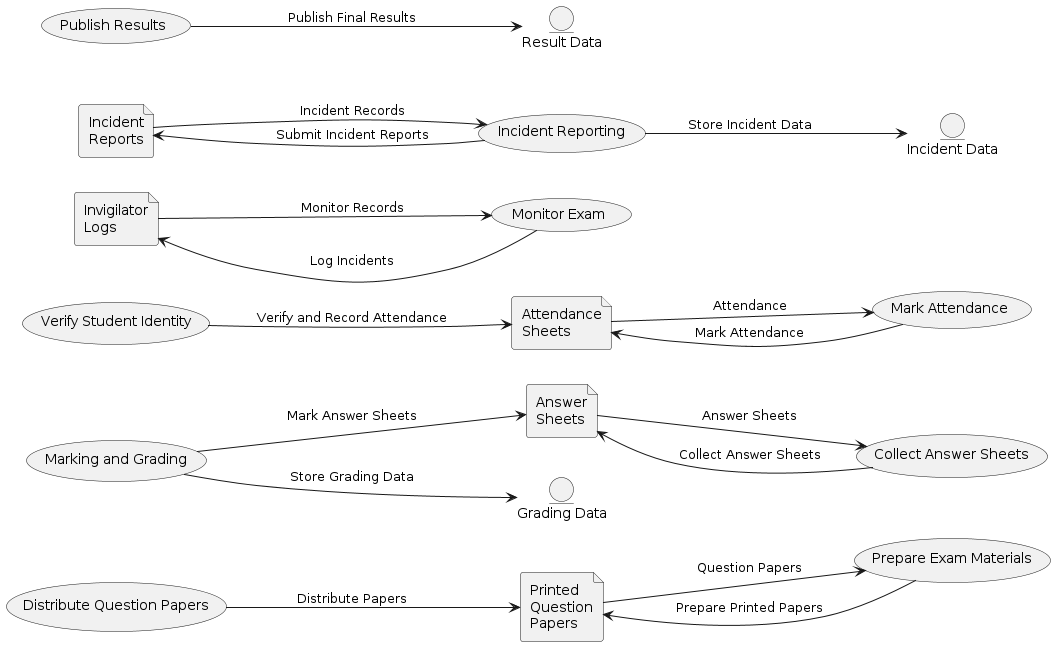
\includegraphics[width=\linewidth]{../figures/dataflow_offline_exam}
	\caption{Dataflow diagram untuk ujian offline.}
	\label{fig:dataflow_offline_exam}
\end{figure}




\subsubsection{Diagram Aliran Data Ujian Offline (Baseline)}

Diagram aliran data untuk sistem ujian offline menunjukkan bagaimana proses ujian dikelola secara manual dengan menggunakan artefak fisik seperti lembar soal, lembar jawaban, dan log pengawas. Berikut adalah penjelasan prosesnya beserta pengkategorian datanya:

\begin{itemize}
	\item \textbf{Dosen} memulai dengan menyiapkan materi ujian, yang kemudian dicetak dan didistribusikan kepada mahasiswa melalui proses "Distribute Question Papers". Hasilnya adalah artefak fisik berupa "Printed Question Papers" (Lembar Soal Cetak).
	\item \textbf{Mahasiswa} memverifikasi identitas mereka, dan kehadiran mereka dicatat dalam "Attendance Sheets" (Lembar Kehadiran) melalui proses "Verify Student Identity" dan "Mark Attendance".
	\item \textbf{Pengawas Ujian} memantau jalannya ujian dan mencatat insiden dalam "Invigilator Logs" (Log Pengawas) melalui proses "Monitor Exam". Jika ada insiden, laporan tersebut dimasukkan dalam "Incident Reports" (Laporan Insiden).
	\item Setelah ujian selesai, lembar jawaban mahasiswa dikumpulkan dalam "Answer Sheets" (Lembar Jawaban) melalui proses "Collect Answer Sheets", yang kemudian digunakan oleh dosen dalam proses penilaian (grading).
	\item \textbf{Dosen} menilai lembar jawaban dan menyimpan hasilnya dalam "Grading Data" (Data Penilaian) melalui proses "Marking and Grading". Setelah penilaian selesai, hasil akhir dipublikasikan melalui proses "Publish Results", yang disimpan dalam "Result Data" (Data Hasil).
	\item Setiap insiden yang dilaporkan selama ujian akan dicatat dalam "Incident Reports" dan datanya disimpan sebagai "Incident Data".
\end{itemize}

\paragraph{Pengkategorian Data Ujian Offline:}
\begin{itemize}
	\item \textbf{Data Fisik:}
	\begin{itemize}
		\item "Printed Question Papers" (Lembar Soal Cetak)
		\item "Answer Sheets" (Lembar Jawaban)
		\item "Attendance Sheets" (Lembar Kehadiran)
		\item "Invigilator Logs" (Log Pengawas)
		\item "Incident Reports" (Laporan Insiden)
	\end{itemize}
	\item \textbf{Data Terstruktur (disimpan dalam database):}
	\begin{itemize}
		\item "Grading Data" (Data Penilaian)
		\item "Result Data" (Data Hasil)
		\item "Incident Data" (Data Insiden)
	\end{itemize}
	\item \textbf{Data Digital Tidak Terstruktur:}
	\begin{itemize}
		\item Tidak relevan untuk sistem ini karena sistem offline mengandalkan artefak fisik.
	\end{itemize}
\end{itemize}

Sistem ini sangat bergantung pada data fisik untuk persiapan dan pengelolaan ujian, sementara hasil penilaian dan data insiden disimpan dalam bentuk data terstruktur yang dapat diakses untuk analisis dan laporan lebih lanjut.

\subsubsection{Diagram Aliran Data Ujian Online (Target)}

\begin{figure}[th!]
	\centering
	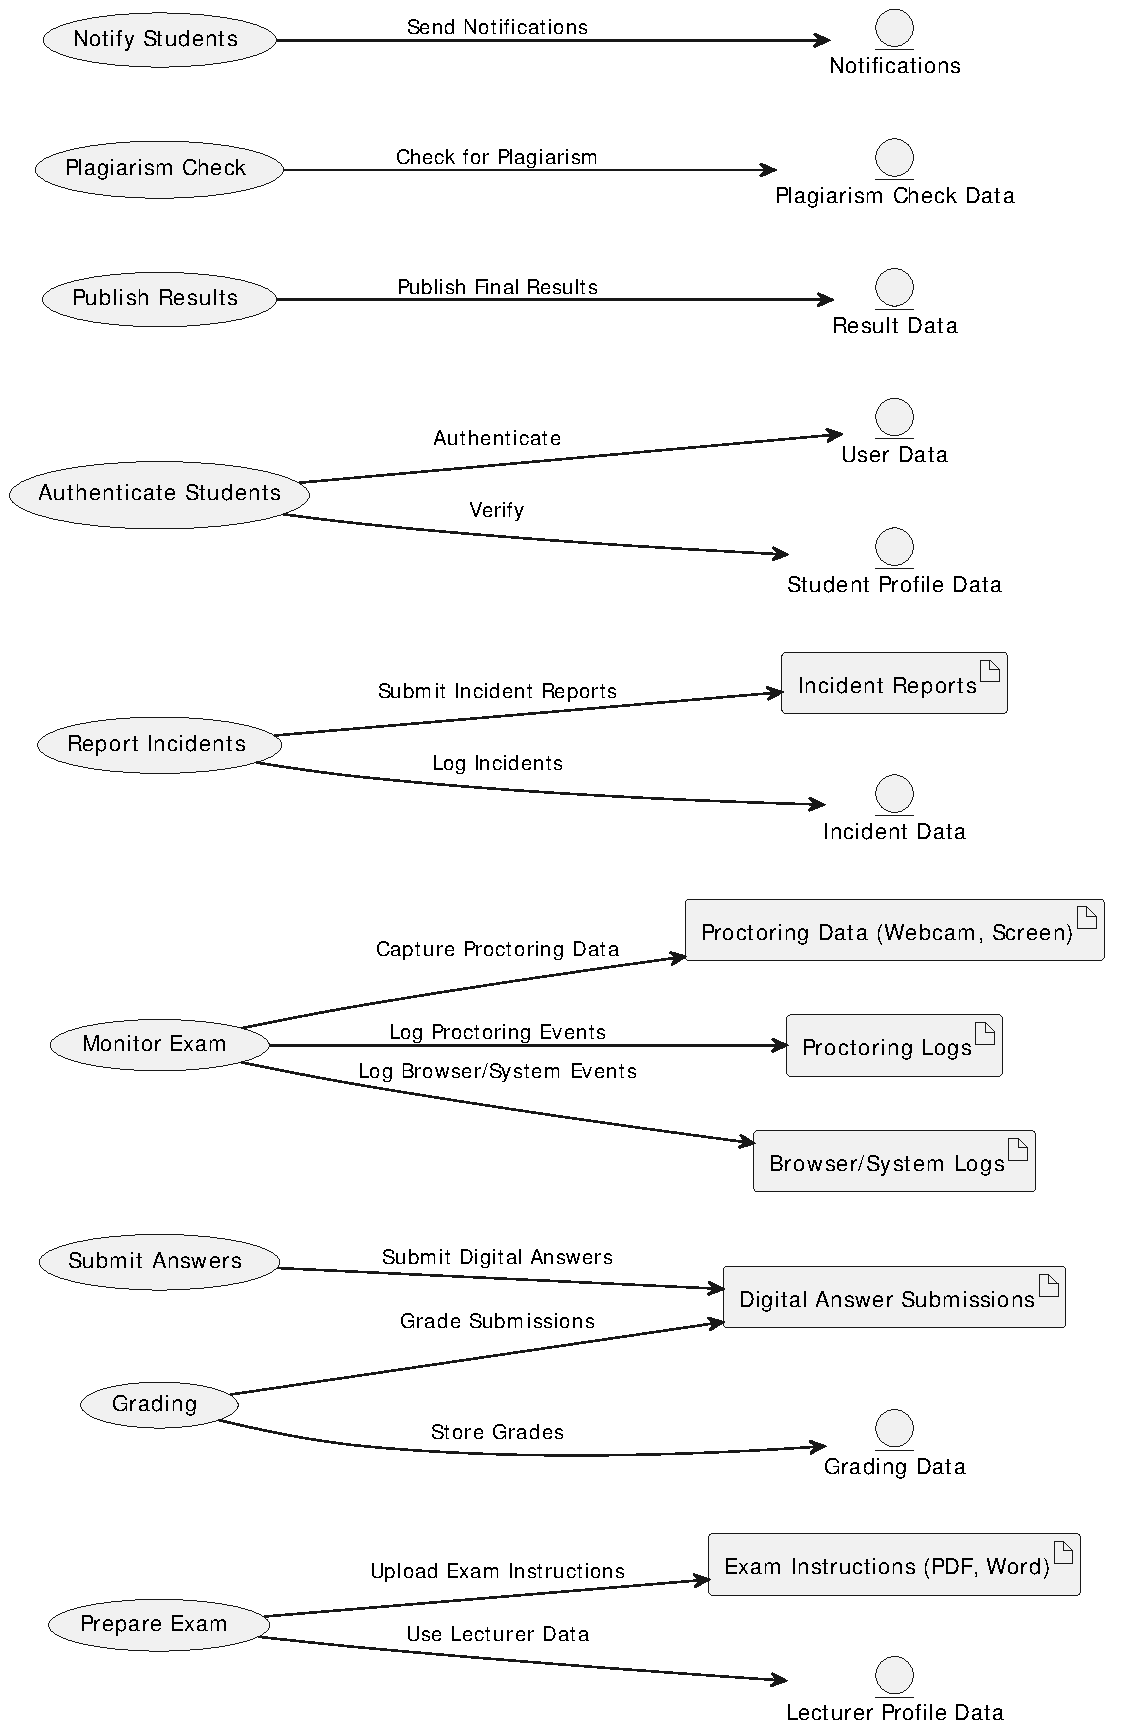
\includegraphics[width=0.7\linewidth]{../figures/dataflow_online_exam}
	\caption{Dataflow diagram untuk ujian online.}
	\label{fig:dataflow_online_exam}
\end{figure}

Diagram aliran data untuk sistem ujian online memperkenalkan otomatisasi dan digitalisasi yang signifikan dalam proses ujian. Berikut adalah penjelasan detailnya, beserta pengkategorian data yang digunakan dalam sistem:

\begin{itemize}
	\item \textbf{Dosen} menyiapkan ujian dengan mengunggah materi ujian, seperti instruksi ujian dalam format PDF atau Word, melalui proses "Prepare Exam". Informasi dosen yang digunakan untuk menyiapkan ujian diambil dari "Lecturer Profile Data".
	\item \textbf{Mahasiswa} harus melakukan autentikasi dan verifikasi identitas melalui proses "Authenticate Students", yang menggunakan data dari "User Data" dan "Student Profile Data".
	\item Selama ujian, \textbf{Platform} memantau aktivitas mahasiswa melalui "Monitor Exam", dengan mengumpulkan data proctoring (misalnya, rekaman webcam atau tangkapan layar) yang disimpan dalam "Proctoring Data", serta mencatat kejadian-kejadian penting dalam "Proctoring Logs". Data dari aktivitas sistem atau browser juga dicatat dalam "Browser/System Logs".
	\item Mahasiswa mengirimkan jawaban ujian secara digital melalui proses "Submit Answers", dan jawaban tersebut disimpan dalam "Digital Answer Submissions".
	\item Setelah pengiriman jawaban, proses "Plagiarism Check" memastikan tidak ada plagiarisme dengan memeriksa data dalam "Plagiarism Check Data". 
	\item \textbf{Dosen} kemudian menilai jawaban mahasiswa melalui proses "Grading", dengan hasil penilaian disimpan dalam "Grading Data". Setelah itu, hasil akhir ujian dipublikasikan melalui "Publish Results" dan disimpan dalam "Result Data".
	\item Mahasiswa menerima pemberitahuan hasil ujian melalui proses "Notify Students", dengan notifikasi yang dikirimkan melalui sistem pemberitahuan dan dicatat dalam "Notifications".
	\item Jika ada insiden selama ujian, laporan insiden tersebut dibuat dalam proses "Report Incidents", dan insiden tersebut dicatat dalam "Incident Reports" serta disimpan sebagai "Incident Data".
\end{itemize}

\paragraph{Pengkategorian Data Ujian Online:}
\begin{itemize}
	\item \textbf{Data Fisik:}
	\begin{itemize}
		\item Tidak ada data fisik, semua proses menggunakan data digital.
	\end{itemize}
	\item \textbf{Data Terstruktur (disimpan dalam database):}
	\begin{itemize}
		\item "User Data" (Data Pengguna)
		\item "Lecturer Profile Data" (Data Profil Dosen)
		\item "Student Profile Data" (Data Profil Mahasiswa)
		\item "Grading Data" (Data Penilaian)
		\item "Result Data" (Data Hasil)
		\item "Incident Data" (Data Insiden)
		\item "Plagiarism Check Data" (Data Pemeriksaan Plagiarisme)
		\item "Notifications" (Pemberitahuan)
	\end{itemize}
	\item \textbf{Data Digital Tidak Terstruktur:}
	\begin{itemize}
		\item "Exam Instructions (PDF, Word)" (Instruksi Ujian)
		\item "Digital Answer Submissions" (Jawaban Digital)
		\item "Proctoring Data (Webcam, Screen)" (Data Proctoring)
		\item "Proctoring Logs" (Log Proctoring)
		\item "Browser/System Logs" (Log Browser/Sistem)
		\item "Incident Reports" (Laporan Insiden)
	\end{itemize}
\end{itemize}

Sistem ujian online bergantung sepenuhnya pada data digital, dengan kombinasi data terstruktur yang disimpan dalam database dan data tidak terstruktur seperti rekaman video, instruksi ujian, dan log sistem yang perlu dikelola secara efisien. Otomatisasi pengelolaan data ini meningkatkan efisiensi, aksesibilitas, dan keamanan dalam mengelola ujian.

Sistem ujian offline bergantung pada penggunaan data fisik, terutama dalam bentuk cetakan dan lembar jawaban, yang memerlukan interaksi manual dan pengelolaan artefak fisik. Sebaliknya, sistem ujian online menggunakan data digital, baik terstruktur maupun tidak terstruktur, yang dikelola secara otomatis oleh platform digital. Sistem online menawarkan efisiensi yang lebih tinggi dan fleksibilitas yang lebih besar dalam manajemen ujian, terutama dalam skenario pembelajaran jarak jauh atau hybrid. Data digital tidak terstruktur seperti rekaman proctoring dan log sistem menjadi elemen penting dalam menjaga integritas dan keamanan ujian online.

\subsection{Analisis Advantages-Disadvantages, Upaya Migrasi, dan Cost-Benefit}

Berdasarkan dataflow diagram untuk ujian offline (baseline) dan online (target), analisis berikut akan membahas kelebihan dan kekurangan dari kedua sistem, langkah-langkah migrasi dari sistem offline ke online, serta analisis biaya-manfaat (cost-benefit) dari transisi ini.

\subsubsection{Analisis Advantages-Disadvantages}

\paragraph{Sistem Ujian Offline (Baseline)}
\textbf{Kelebihan:}
\begin{itemize}
	\item Tidak memerlukan infrastruktur teknologi yang kompleks, sehingga tidak ada ketergantungan pada perangkat digital atau jaringan internet.
	\item Proses sudah dikenal oleh para dosen, pengawas, dan mahasiswa, sehingga tidak memerlukan pelatihan tambahan.
	\item Pengawasan fisik secara langsung (oleh pengawas) dapat lebih mudah mengatasi kecurangan yang jelas terlihat.
\end{itemize}

\textbf{Kekurangan:}
\begin{itemize}
	\item Proses manual memerlukan banyak waktu dan sumber daya (misalnya mencetak soal, mengumpulkan lembar jawaban).
	\item Rentan terhadap kesalahan manusia, baik dalam pencatatan kehadiran, pengumpulan, maupun penilaian.
	\item Pengelolaan insiden (seperti laporan insiden di ruang ujian) memerlukan dokumentasi fisik yang bisa hilang atau rusak.
	\item Skalabilitas terbatas, terutama untuk ujian dengan jumlah mahasiswa yang besar atau pada situasi pembelajaran jarak jauh.
\end{itemize}

\paragraph{Sistem Ujian Online (Target)}
\textbf{Kelebihan:}
\begin{itemize}
	\item Otomatisasi proses seperti pengumpulan jawaban, pengecekan plagiarisme, dan publikasi hasil ujian mengurangi waktu dan sumber daya yang dibutuhkan.
	\item Lebih aman dan efisien dalam pengelolaan data, baik untuk penyimpanan hasil ujian, laporan insiden, maupun pemantauan aktivitas mahasiswa.
	\item Mendukung fleksibilitas bagi mahasiswa yang mengikuti ujian dari jarak jauh atau dalam situasi hybrid.
	\item Data digital seperti log pengawasan dan data proctoring dapat digunakan untuk mengurangi risiko kecurangan dan meningkatkan transparansi.
\end{itemize}

\textbf{Kekurangan:}
\begin{itemize}
	\item Memerlukan infrastruktur teknologi yang handal, termasuk jaringan internet, perangkat keras, dan perangkat lunak yang mendukung.
	\item Risiko keamanan siber, seperti potensi kebocoran data pribadi atau gangguan teknis yang dapat mengganggu proses ujian.
	\item Kurva pembelajaran untuk dosen, mahasiswa, dan pengawas dalam mengoperasikan sistem ujian digital dan pemantauan online.
\end{itemize}

\subsubsection{Upaya Migrasi dari Ujian Offline (Baseline) ke Ujian Online (Target)}

Migrasi dari sistem ujian offline ke sistem ujian online memerlukan beberapa upaya yang meliputi:

\begin{enumerate}
	\item \textbf{Penyiapan Infrastruktur Teknologi:}
	\begin{itemize}
		\item Pengadaan platform ujian online, perangkat keras, dan jaringan yang mendukung kelancaran ujian online.
		\item Menyiapkan ruang server dan penyimpanan untuk menangani data digital besar seperti rekaman proctoring, log sistem, dan hasil ujian.
	\end{itemize}
	\item \textbf{Pelatihan dan Familiarisasi:}
	\begin{itemize}
		\item Melatih dosen, mahasiswa, dan pengawas dalam penggunaan platform ujian, termasuk cara menggunakan proctoring dan pengecekan plagiarisme.
		\item Menyediakan panduan dan simulasi ujian online untuk memastikan semua pihak terbiasa dengan sistem baru.
	\end{itemize}
	\item \textbf{Keamanan dan Kebijakan Penggunaan:}
	\begin{itemize}
		\item Mengembangkan kebijakan keamanan data dan protokol dalam menangani masalah teknis serta potensi kecurangan digital.
		\item Menerapkan prosedur yang jelas untuk menangani insiden yang terkait dengan pemantauan dan proctoring secara online.
	\end{itemize}
	\item \textbf{Uji Coba dan Pengawasan:}
	\begin{itemize}
		\item Melakukan uji coba sistem ujian online dengan kelompok kecil untuk memastikan bahwa sistem berjalan dengan baik tanpa masalah teknis.
		\item Menerapkan sistem pemantauan dan audit terhadap proses ujian online untuk memastikan integritas dan keamanan ujian.
	\end{itemize}
\end{enumerate}

\subsubsection{Analisis Cost-Benefit}

\paragraph{Biaya:}
\begin{itemize}
	\item \textbf{Pengadaan Teknologi:} Pengeluaran awal yang signifikan untuk pengadaan platform ujian online, perangkat keras tambahan, server, serta perangkat proctoring.
	\item \textbf{Pelatihan:} Biaya untuk pelatihan staf pengajar, pengawas, dan mahasiswa dalam penggunaan sistem baru, serta pembuatan materi panduan.
	\item \textbf{Pemeliharaan dan Dukungan Teknis:} Biaya berkelanjutan untuk pemeliharaan sistem, dukungan teknis, serta pembaruan perangkat lunak dan keamanan.
	\item \textbf{Keamanan dan Perlindungan Data:} Pengeluaran tambahan untuk memastikan keamanan data mahasiswa dan mencegah potensi ancaman siber.
\end{itemize}

\paragraph{Manfaat:}
\begin{itemize}
	\item \textbf{Efisiensi Waktu dan Biaya Operasional:} Otomatisasi proses pengumpulan, penilaian, dan publikasi hasil ujian mengurangi beban kerja manual dan waktu pemrosesan.
	\item \textbf{Aksesibilitas dan Skalabilitas:} Mahasiswa dapat mengikuti ujian dari lokasi mana pun, sehingga mendukung pembelajaran jarak jauh dan hybrid. Sistem ini juga mampu menangani jumlah mahasiswa yang lebih besar secara efisien.
	\item \textbf{Pengelolaan Data yang Lebih Baik:} Penyimpanan digital memudahkan pengelolaan data secara terpusat dan memastikan transparansi hasil ujian serta catatan insiden.
	\item \textbf{Peningkatan Keamanan Ujian:} Penggunaan proctoring digital, log aktivitas, dan pengecekan plagiarisme meningkatkan integritas dan keadilan dalam pelaksanaan ujian.
\end{itemize}

Walaupun terdapat biaya awal yang cukup besar dalam implementasi sistem ujian online, manfaat jangka panjang seperti efisiensi, aksesibilitas, dan peningkatan keamanan menjadikannya solusi yang sangat bermanfaat. Selain itu, sistem online memungkinkan pengelolaan ujian secara lebih fleksibel dan terstruktur, terutama dalam skenario pembelajaran jarak jauh.


\section{Aktivitas Kelas dan Tugas}
Buat model data dan dokumen \textbf{As-Is} yang terpengaruh oleh kapabilitas yang dipilih. Selain itu, buat model data dan dokumen \textbf{To-Be} yang diperlukan untuk mewujudkan kapbilitas terpilih. Tuangkan dalam bentuk atau perbaharui Dokumen Definisi Arsitektur (Subbab \ref{sec:isi_dokumen_definisi_arsitektur} dan \ref{sec:dokumen_definisi_arsitektur_data}) dan Spesifikasi Persyaratan Arsitektur (Subbab \ref{sec:spesifikasi_kebutuhan_arsitektur} dan  \ref{sec:spesifikasi_kebutuhan_arsitektur_data}).
